
\chapter{누적분포함수}
\label{cumulative}

이번 장에서 사용되는 코드는 {\tt cumulative.py}에 있다.
코드를 다운로드하고 작업하는 것에 대한 정보는 ~\ref{code}을 참조한다.


\section{PMF의 한계점}
\index{PMF}

PMF는 값(value)의 수가 작다면 잘 동작한다. 하지만, 값의 갯수가 증가함에 따라,
각 값과 연관된 확률값이 더 작아지고 확률잡음(random noise)의 효과는 증가한다.

예를 들어, 출산 체중 분포에 관심이 있다고 하자. NSFG 데이터에서 
\verb"totalwgt_lb" 변수가 파운드로 출생 체중을 기록한다.
그림~\ref{nsfg_birthwgt_pmf}이 첫번째 아이와 첫째가 아닌 아이에 대한 체중값을 
PMF로 보여준다.
\index{가족 성장 국가 조사 (National Survey of Family Growth)} 
\index{NSFG} 
\index{출산 체중 (birth weight)}
\index{체중 (weight)!출산 (birth)}

\begin{figure}
% cumulative.py
%\centerline{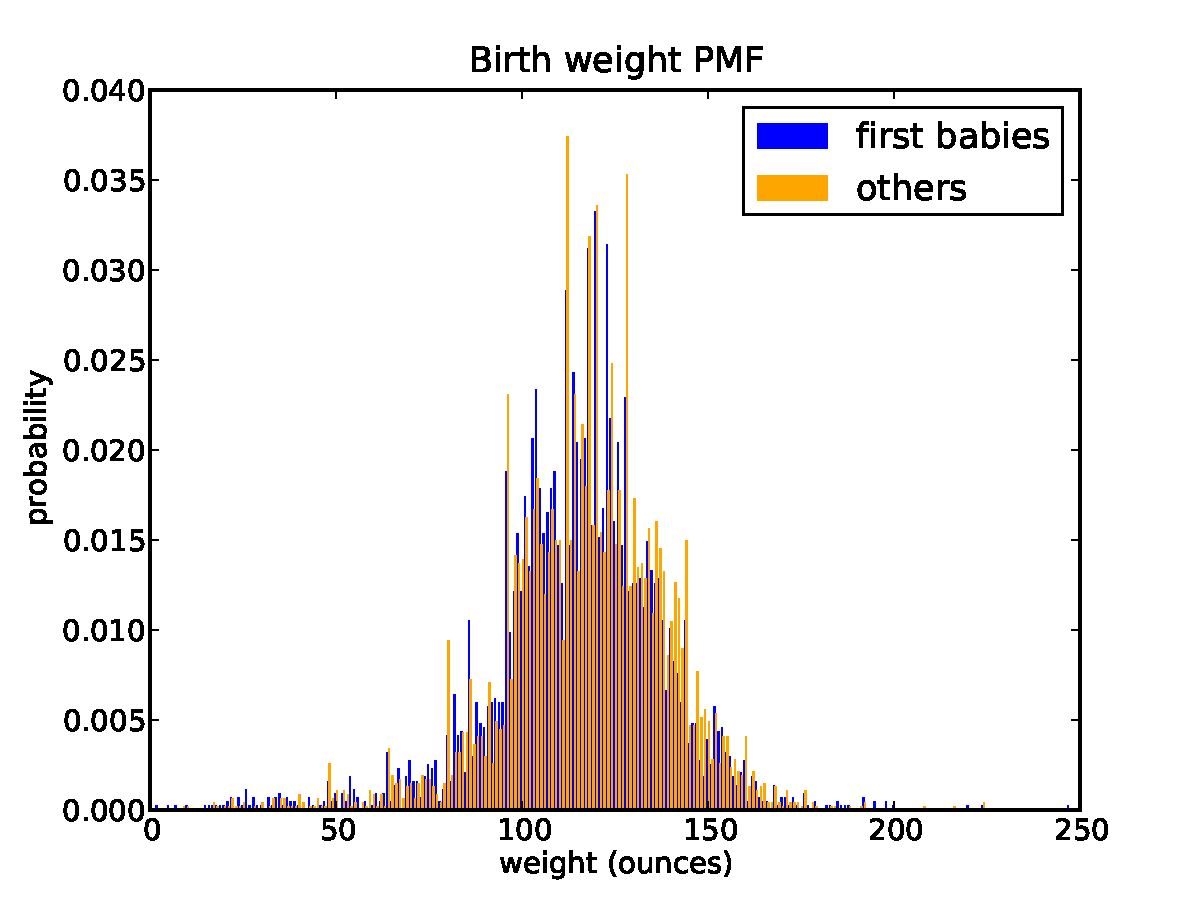
\includegraphics[height=2.5in]{figs/nsfg_birthwgt_pmf.pdf}}
\caption{PMF of birth weights.  This figure shows a limitation
of PMFs: they are hard to compare visually.}
\label{nsfg_birthwgt_pmf}
\end{figure}

전반적으로 분포는 정규분포의 종모양을 닮았다.
평균 근처에 값이 많고 체중이 더 높거나 더 낮아지면 값이 작아진다.

하지만 그림을 이해하기는 어렵다. 뾰족한 것과 골자기가 많고, 두 집단 분포 사이에
명백한 차이도 보인다. 여럿중에서 어느 면이 유의미한지 분간하기는 쉽지 않다.
또한 전반적인 패턴을 보기도 어렵다; 예를 들어, 여러분이 보기에 어느 분포가 평균값이 더 높은가?
\index{통에 담기(binning)}

데이터를 구간(bin)에 담는 것으로 이러한 문제는 완화될 수 있다; 즉, 값 범위를 서로 겹쳐지지 않는 구간으로 
나누고 각 구간(bin)에 값 갯수를 계수한다. 구간에 담는 것(binning)은 유용하지만,
적정한 구간 크기를 잡는 것은 까다롭다. 잡음을 평활(smooth out)하기 위해서 충분히 큰 통을 잡는 것이 
또한 유용한 정보도 평활할 수도 있다.

이러한 문제를 회피하는 대안이 누적분포함수(cumulative
distribution function, CDF)로 이번 장 학습주제다. 하지만, CDF를 설명하기 전에 백분위수(percentile)를 먼저 설명해야 한다.
\index{CDF}


\section{백분위수 (Percentiles)}
\index{백분위 순위 (percentile rank)}

만약 전국 단위 표준시험을 치르게 되면, 원점수와 {\bf 백분위 순위(percentile rank)} 형태로 시험결과를 받아보게 된다. 이러한 맥락에서 백분위 순위는 시험 당사자보다 적은 점수를 얻는 사람들이 된다.
그래서 만약 ``백분위수 90번째''라면, 시험을 치른 90\% 사람보다 혹은 동등하다는 의미가 된다.

다음에 {\tt scores} 시퀀스 값에서 상대적으로 \verb"your_score" 값에 대한 백분위 순위를 계산하는 방법이 있다.

%
\begin{verbatim}
def PercentileRank(scores, your_score):
    count = 0
    for score in scores:
        if score <= your_score:
            count += 1

    percentile_rank = 100.0 * count / len(scores)
    return percentile_rank
\end{verbatim}

예제로 만약 시퀀스 점수가 55, 66, 77, 88, 99이고, 시험 점수로 88점을 받았다면, 
백분위 순위는 {\tt 100 * 4 / 5}, 80이 된다.

값이 주어진다면, 백분위 순위를 찾기는 쉽다; 반대 방향으로는 다소 더 어렵다.
만약 백분위 순위가 주어진 상태에서 해당하는 값을 찾고자 한다면, 한 선택지는 값을 정렬하고
원하는 값을 찾는 것이다.

%
\begin{verbatim}
def Percentile(scores, percentile_rank):
    scores.sort()
    for score in scores:
        if PercentileRank(scores, score) >= percentile_rank:
            return score
\end{verbatim}

계산 결과는 {\bf 백분위수(percentile)}가 된다. 
예를 들어, 50번째 백분위 수는 백분위 순위가 50 인 값이 된다. 
시험점수 분포에서 50번째 백분위 수는 77이다.
\index{백분위수 (percentile)}

{\tt Percentile} 구현코드가 그다지 효율적이지 않다.
더 나은 접근법은 백분위 순위를 사용해서 해당하는 백분위수 인덱스를 계산하는 것이다.

\begin{verbatim}
def Percentile2(scores, percentile_rank):
    scores.sort()
    index = percentile_rank * (len(scores)-1) // 100
    return scores[index]
\end{verbatim}

``백분위수 (percentile)''와 ``백분위 순위 (percentile rank)'' 차이가 혼동스러울 수 있고
항상 용어를 정확하게 구별하여 사용하지는 않는다. 요약하면,
{\tt PercentileRank} 함수는 값을 인자로 받아 값 집합에서 백분위 순위를 계산한다;
{\tt Percentile} 함수는 백분위 순위를 인자로 받아 해당하는 값을 계산한다. 
\index{백분위 순위 (percentile rank)}

\section{CDF}
\index{CDF}

이제 백분위수와 백분위 순위를 이해하고 있기 때문에, {\bf 누적분포함수(cumulative distribution function, CDF)}를 다룰 준비가 되었다. CDF는 값을 백분위 순위로 매핑하는 함수다.
\index{누적분포함수 (cumulative distribution function)}
\index{백분위 순위 (percentile rank)}

CDF는 $x$의 함수로 $x$는 분포에 나타나는 임의값이다.  
특정한 $x$ 값에 대해서 $\CDF(x)$를 평가하기 위해서, 
$x$와 동일하거나 작은 분포의 분수값을 계산한다.

시퀀스 {\tt sample}와 값 {\tt x}를 인자로 받는 함수로 어떤 느낌인지 다음에 코드가 있다.

%
\begin{verbatim}
def EvalCdf(sample, x):
    count = 0.0
    for value in sample:
        if value <= x:
            count += 1

    prob = count / len(sample)
    return prob
\end{verbatim}

함수가 거의 {\tt PercentileRank}과 동일하지만, 백분위 순위가 0--100인 반면에 결과값이 0--1 범위를 갖는 확률이라는 점이 차이가 있다.
\index{표본 (sample)}

예제로 표본값으로 {\tt [1, 2, 2, 3, 5]}을 수집했다고 가정하자. 다음에 CDF로부터 값이 몇개 있다.
%
\[ CDF(0) = 0 \]
%
\[ CDF(1) = 0.2\]
%
\[ CDF(2) = 0.6\]
%
\[ CDF(3) = 0.8\]
%
\[ CDF(4) = 0.8\]
%
\[ CDF(5) = 1\]
%

표본에 있는 값뿐만 아니라 $x$의 임의값에 대해서 CDF를 평가할 수 있다.
만약 $x$가 표본에 가장 작은 값보다 작다면, $\CDF(x)$는 0.
만약 $x$가 가장 큰 값보다 크다면, $\CDF(x)$는 1.

\begin{figure}
% cumulative.py
%\centerline{\includegraphics[height=2.5in]{figs/cumulative_example_cdf.pdf}}
\caption{Example of a CDF.}
\label{example_cdf}
\end{figure}

그림~\ref{example_cdf}이 CDF를 그래픽으로 표현한 것이다.
표본 CDF는 계단 함수다.
\index{계단 함수 (step function)}


\section{CDF 표현하기 (Representing CDFs)}
\index{Cdf}

{\tt thinkstats2}은 CDF를 표현하는 Cdf라는 클래스를 제공한다. Cdf 가 제공하는 기본 메쏘드는 다음과 같다.

\begin{itemize}

\item {\tt Prob(x)}: {\tt x} 값이 주어졌을 때, $p = \CDF(x)$ 확률값을 계산한다. 꺾쇠 연산자는 {\tt Prob}와 동일하다.
\index{꺾쇠 연산자 (bracket operator)}

\item {\tt Value(p)}: 확률 {\tt p}가 주어졌을 때, 
상응하는 값 {\tt x}를 계산한다; 즉, {\tt p}의 {\bf CDF 역함수(inverse CDF)}다.
\index{CDF 역함수 (inverse CDF)}
\index{CDF, 역함수(inverse)}

\end{itemize}

\begin{figure}
% cumulative.py
%\centerline{\includegraphics[height=2.5in]{figs/cumulative_prglngth_cdf.pdf}}
\caption{CDF of pregnancy length.}
\label{cumulative_prglngth_cdf}
\end{figure}

Cdf 생성자는 인자로 리스트, 판다스 시리즈, Hist, Pmf, 혹은 또다른 Cdf를 받을 수 있다. NSFG 데이터에서 임신 기간 분포에 대한 Cdf를 생성하는 코드가 다음에 있다. 

\index{NSFG}
\index{임신 기간 (pregnancy length)}

\begin{verbatim}
    live, firsts, others = first.MakeFrames()
    cdf = thinkstats2.Cdf(live.prglngth, label='prglngth')
\end{verbatim}


{\tt thinkplot}은 {\tt Cdf}라는 함수를 제공해서 Cdf를 선그래프를 그릴 수 있다.
\index{thinkplot}

\begin{verbatim}
    thinkplot.Cdf(cdf)
    thinkplot.Show(xlabel='weeks', ylabel='CDF')
\end{verbatim}



그림~\ref{cumulative_prglngth_cdf}에 결과가 있다.
CDF를 읽는 한가지 방법은 백분위수를 찾는 것이다.
예를 들어, 임신 기간 10\%는 36주차보다 더 짧고, 90\%는 41주차보다 더 짧은 것처럼 보인다. 또는 CDF를 통해서 분포 모양을 시각적으로 표현할 수도 있다. 흔한 값은 CDF에서 급격하거나 수직적 부분으로 나타난다; 이번 예제에서 39주차 모드(최빈값)가 명확히 보인다. 30주차 밑으로 값이 몇개 없어서 이 범위에 있는 CDF는 평평하다.
\index{CDF, 해석하기 (interpreting)}

CDF에 익숙해지는데 시간이 좀 필요하다. 하지만, 한번 익숙해지면, PMF보다 더 많은 정보를 좀더 명확하게 보여줄 것으로 생각된다.


\section{CDF 비교하기}
\label{birth_weights}
\index{가족 성장 국가 조사 (National Survey of Family Growth)}
\index{NSFG}
\index{출산 체중 (birth weight)}
\index{체중 (weight)!출산 (birth)}

CDF는 특히 분포를 비교하는데 유용하다.
예를 들어, 첫째 아이와 첫째 아이가 아닌 아이에 대한 출산 체중 CDF를 플롯으로 그리는 코드가 다음에 있다.
\index{thinkplot}
\index{분포 (distributions), 비교하기 (comparing)}

\begin{verbatim}
    first_cdf = thinkstats2.Cdf(firsts.totalwgt_lb, label='first')
    other_cdf = thinkstats2.Cdf(others.totalwgt_lb, label='other')

    thinkplot.PrePlot(2)
    thinkplot.Cdfs([first_cdf, other_cdf])
    thinkplot.Show(xlabel='weight (pounds)', ylabel='CDF')
\end{verbatim}

\begin{figure}
% cumulative.py
%\centerline{\includegraphics[height=2.5in]{figs/cumulative_birthwgt_cdf.pdf}}
\caption{CDF of birth weights for first babies and others.}
\label{cumulative_birthwgt_cdf}
\end{figure}

그림~\ref{cumulative_birthwgt_cdf}에 결과가 있다.
그림~\ref{nsfg_birthwgt_pmf}와 비교하여, 좀더 명확하게 분포 모양과 분포간의 차이를 그림에서 보여준다.
첫째 아이 체중이 평균 이상에서 조금더 커다란 불일치성을 보이고, 분포 전반에 걸쳐 다소 가볍다는 것을 볼 수 있다.

\index{모양 (shape)}

\section{백분위수 기반 통계량 (Percentile-based statistics)}
\index{요약 통계 (summary statistic)}
\index{사분위수 범위 (interquartile range)}
\index{분위수 (quartile)}
\index{백분위수 (percentile)}
\index{중위수 (median)}
\index{중심 경향성 (central tendency)}
\index{퍼짐 (spread)}

CDF를 계산하게 되면, 백분위수와 백분위 순위를 계산하기는 쉽다.
Cdf 클래스가 두가지 메쏘드를 제공한다.
\index{Cdf}
\index{백분위 순위 (percentile rank)}

\begin{itemize}

\item {\tt PercentileRank(x)}: {\tt x}가 주어지면, $100 \cdot \CDF(x)$ 백분위 순위를 계산한다.

\item {\tt Percentile(p)}: 백분위 순위 {\tt rank}가 주어지면,
해당하는 값 {\tt x}를 계산한다. {\tt Value(p/100)}과 동등하다.

\end{itemize}

{\tt 백분위수 (Percentile)}는 백분위수 기반 요양 통계량을 계산하는데 사용될 수 있다. 예를 들어 50번째 백분위수는 {\bf 중위수 (median)}로 알려진 분포를 반으로 나누는 값이다. 평균과 마찬가지로 중위수는 분포의 중심경향성을 측정하는 측도다.

사실, 각기 다른 특성을 가진 ``중위수(median)''에 대한 정의가 몇개 있다. 하지만, {\tt Percentile(50)}가 단순하고 계산하기 효율적이다.

또 다른 백분위수 기반 통계량이 {\bf 사분위수 범위 (interquartile range, IQR}로 분포의 퍼짐을 측정하는 측도다.
IQR는 75번째와 25번째 백분위수 간의 차이다.

좀더 일반적으로, 백분위수는 종종 분포 모양을 요약하는데 쓰여진다.
예를 들어, 수입 분포는 종종 ``분위수 (quintiles)''로 보고된다; 즉, 20번째, 40번째, 60번째, 80번째 백분위수로 쪼개진다.
다른 분포는 10개 ``십분위(deciles)''으로 나눠진다.
이와 같이 CDF에서 동일간격으로 표현되는 통계량을 {\bf 분위수(quantiles)}라고 한다. 좀더 자세한 정보는 다음 웹사이트를 참고 바란다. \url{https://en.wikipedia.org/wiki/Quantile}.
\index{분위수 (quantile)}
\index{오분위수 (quintile)}
\index{십분위수 (decile)}


\section{난수 (Random numbers)}
\label{random}
\index{난수 (random number)}

정상 출산 모집단에서 임의 표본을 추출하고, 출생 체중 백분위 순위를 찾아낸다고 가정하자. 이제 백분위 순위 CDF를 계산한다고 가정하자.
분포가 어떨 것으로 생각하는가?

\index{백분위 순위 (percentile rank)}
\index{출생 체중 (birth weight)}
\index{체중 (weight)!출생 (birth)}

다음에 어떻게 계산하는지 코드가 있다. 첫째로 출생 체중 Cdf를 생성한다.
\index{Cdf}

\begin{verbatim}
    weights = live.totalwgt_lb
    cdf = thinkstats2.Cdf(weights, label='totalwgt_lb')
\end{verbatim}

그리고 나서, 표본을 생성하고, 표본에 있는 각 값에 대한 백분위 순위를 계산한다.

\begin{verbatim}
    sample = np.random.choice(weights, 100, replace=True)
    ranks = [cdf.PercentileRank(x) for x in sample]
\end{verbatim}

{\tt sample}은 100개 출생 체중 임의 표본이며 복원 추출하였다;
즉, 동일한 값이 한번이상 추출될 수 있다. 
{\tt ranks}는 백분위 순위 리스트다.
\index{복원 (replacement)}

마지막으로 백분위 순위 Cdf를 만들고 플롯으로 그린다.

\index{thinkplot}

\begin{verbatim}
    rank_cdf = thinkstats2.Cdf(ranks)
    thinkplot.Cdf(rank_cdf)
    thinkplot.Show(xlabel='percentile rank', ylabel='CDF')
\end{verbatim}

\begin{figure}
% cumulative.py
%\centerline{\includegraphics[height=2.5in]{figs/cumulative_random.pdf}}
\caption{CDF of percentile ranks for a random sample of birth weights.}
\label{cumulative_random}
\end{figure}

그림~\ref{cumulative_random}이 결과를 보여준다.
CDF가 근사적으로 직선이다. 분포가 균등하다라는 의미다. 

결과가 명확하지 않을 수도 있지만, CDF가 정의된 방식의 결과다.
그림이 보여주는 정보는 표본의 10\%가 10번째 백분위수 보다 밑에 있고,
표본의 20\%가 20번째 백분위수 보다 밑에 있고 등등, 정확히 예측했던 것이다.

그래서, CDF 모양에 관계없이, 백분위 순위 분포는 균등하다. 
이 속성이 유용한데, 이유는 주어진 CDF에서 난수를 생성하는데 있어서 간단하면서도 효율적인 알고리즘 설계하는 기초가 되기 때문이다; 다음에 난수를 생성하는 방법이 있다.

\index{역 CDF 알고리즘 (inverse CDF algorithm)}
\index{난수 (random number)}

\begin{itemize}

\item 0--100 범우에서 균등하게 백분위 순위를 고른다.

\item {\tt Cdf.Percentile}를 사용해서 선택한 백분위 순위에 상응하는 값을 분포에서 찾는다.
\index{Cdf}

\end{itemize}

Cdf는 상기 알고리즘을 구현한 것으로 {\tt Random}이 함수명이다.

\begin{verbatim}
# class Cdf:
    def Random(self):
        return self.Percentile(random.uniform(0, 100))
\end{verbatim}

Cdf는 {\tt Sample} 메쏘드를 제공하는데 정수 {\tt n}을
인자로 받아 Cdf에서 임의로 추출한 {\tt n}개 리스트를 반환한다.


\section{백분위 순위 비교하기}

백분위 순위는 다른 집단에 대해서 측정값을 비교하는데 유용하다.
예를 들어, 달리기 경주에서 참가자는 대체로 나이와 성별로 무리를 만든다.
다른 연령 집단에 있는 사람을 비교하는데 경주시간을 백분위 순위로 변환할 수 있다.

\index{백분위 순위 (percentile rank)}

몇년전에 매사추세츠(Massachusetts)주에서 제임스 조이스(James Joyce) 10킬로 마라톤을 뛰었다;
42분 44초로 주파해서 1633명중에서 97번째로 완주했다. 참가자 1633명 중 1537명 참가자보다 빨리 도착해서 
저자의 최종 백분위 순위는 94\%다.  
\index{제임스 조이스 마라톤 (James Joyce Ramble} 
\index{경주 시간 (race time)}


좀더 일반적으로, 위치와 필드 크기 정보가 주어진다면, 백분위 순위를 계산할 수 있다.
\index{필드 크기 (field size)}

\begin{verbatim}
def PositionToPercentile(position, field_size):
    beat = field_size - position + 1
    percentile = 100.0 * beat / field_size
    return percentile
\end{verbatim}

``40에서 49세 남성'', M4049로 표기된 저자가 속한 연령집단, 256명 중에서 26번째로 완주했다.
그래서, 저자가 속한 연령집단에서 백분위 순위는 90\%가 된다.
\index{연령 집단 (age group)}

10년정도 더 마라톤을 뛴다면 (그리고 계속해서 뛰고 싶다.), M5059 그룹에 있을 것이다.
저자가 속한 집단에서 동일한 백분위수를 유지한다고 가정한다면, 완주하는데 얼마나 더 시간이 필요할까?

M4049 집단에 있는 저자의 백분위 순위를 M5059 집단에 위치로 전환하면 상기 질문에 대답할 수 있다.
다음에 프로그램 코드가 있다.

\begin{verbatim}
def PercentileToPosition(percentile, field_size):
    beat = percentile * field_size / 100.0
    position = field_size - beat + 1
    return position
\end{verbatim}

M5059 집단에 171 명이 있어서 동일한 백분위 순위를 유지하려면 17번째와 18번째 사이에서 완주해야 한다.
M5059에서 17번째 마라토너가 46:05로 완주해서, 40대 동일한 백분위 순위를 유지하는데 
46:05 시간이 완주 목표시간이 된다.


\section{Exercises}

For the following exercises, you can start with \verb"chap04ex.ipynb".
My solution is in \verb"chap04soln.ipynb".

\begin{exercise}
How much did you weigh at birth?  If you don't know, call your mother
or someone else who knows.  Using the NSFG data (all live births),
compute the distribution of birth weights and use it to find your
percentile rank.  If you were a first baby, find your percentile rank
in the distribution for first babies.  Otherwise use the distribution
for others.  If you are in the 90th percentile or higher, call your
mother back and apologize.
\index{birth weight}
\index{weight!birth}

\end{exercise}

\begin{exercise}
The numbers generated by {\tt random.random} are supposed to be
uniform between 0 and 1; that is, every value in the range
should have the same probability.

Generate 1000 numbers from {\tt random.random} and plot their
PMF and CDF.  Is the distribution uniform?
\index{uniform distribution}
\index{distribution!uniform}
\index{random number}

\end{exercise}


\section{용어사전}

\begin{itemize}

\item 백분위 순위 (percentile rank): 
분포에서 주어진 값과 동일하거나 적은 값의 퍼센티지.
\index{백분위 순위 (percentile rank)}

\item 백분위수 (percentile): 주어진 백분위 순위와 연관된 값.
\index{백분위수 (percentile)}

\item 누적분포함수 (cumulative distribution function, CDF): 
값에서 누적확률값으로 매핑하는 함수. $\CDF(x)$는 $x$와 동일하거나 작은 표본비율이다. 
\index{CDF}
\index{누적 확률 (cumulative probability)}

\item 역 CDF (inverse CDF):
누적 확률($p$)에서 해당값으로 매핑하는 함수.
\index{역 CDF (inverse CDF)}
\index{CDF, 역 (inverse)}

\item 중위수 (median): 
종종 중심경향성 측도로 사용되는 50번째 백분위수.
\index{중위수 (median)}

\item 사분위 범위 (interquartile range): 
퍼짐의 측도로 사용되는 75번째와 25번째 백분위수 간 차이.
\index{사분위 범위 (interquartile range)}

\item 분위수 (quantile): 
동일 간격 백분위 순위에 상응하는 스퀀스 값; 예를 들어, 
분포 사분위수는 25번째, 50번째, 75번째 백분위수가 된다.
\index{분위수 (quantile)}

\item 복원 (replacement): 
표본추출 과정의 속성. ``복원추출 (With replacement)''는 동일한 값이 한번이상 추출될 수 있다는 의미다;
``비복원추출 (Without replacement)''는 값이 한번 추출될면, 모집단에서 제거된다는 의미가 된다.
\index{복원 (replacement)}

\end{itemize}

